\chapter{Fits of the strong coupling constant}
\label{sec:Fits}

As discussed in the previous section, the measured inclusive 2-jet and 3-jet event cross sections and their ratio \ratio can be used for a determination of the strong coupling constant \alpsmz. The value of \alpsmz is determined by minimizing the \chisq between the experimental measurement and the theoretical predictions. The fit procedure here follows closely the one previously used in Refs.~\cite{Chatrchyan:2013txa} and~\cite{Khachatryan:2014waa}. The \chisq is defined as:

\begin{equation}
  \label{chisq}
  \chisq = M^{T}C^{-1}M\,,
\end{equation}

where $M$ is the vector of the differences between the data ($D^{i}$) and the theoretical values ($T^{i}$) in each bin $i$,

\begin{equation}
  \label{eqn:M_matrix}
  M^{i}=D^{i}-T^{i}
\end{equation}

and $C$ is the covariance matrix including all experimental uncertainties as described in Section~\ref{sec:Measurement} and some theoretical uncertainties. More precisely, $C=C_\mathrm{exp}+C_\mathrm{theo}$ is defined as the sum of covariances of experimental and theoretical sources of uncertainty as follows

\begin{eqnarray}
  \label{eqn:c_exp}
  C_\mathrm{exp} &=& \mathrm{Cov}^\mathrm{ExpStat} + \sum\mathrm{Cov}^\mathrm{JEC} +
  \mathrm{Cov}^\mathrm{Unfolding} +
  % \mathrm{Cov}^\mathrm{JER} +
  \mathrm{Cov}^\mathrm{Lumi} +
  \mathrm{Cov}^\mathrm{Uncor}\,,\\
  C_\mathrm{theo} &=& \mathrm{Cov}^\mathrm{TheoStat} + \mathrm{Cov}^\mathrm{NP} + \mathrm{Cov}^\mathrm{PDF}\,,
  \label{eqn:c_theo}
\end{eqnarray}

where the labelled covariance matrices account for the following effects:

\begin{itemize}
\item{$\mathrm{Cov}^\mathrm{ExpStat}$: the statistical uncertainty of the
    data including correlations introduced by the unfolding,}
\item{$\mathrm{Cov}^\mathrm{JEC}$: the JEC
systematic uncertainty,}
\item{$\mathrm{Cov}^\mathrm{Unfolding}$: the unfolding systematic
    uncertainty including the JER,}
\item{$\mathrm{Cov}^\mathrm{Lumi}$: the luminosity uncertainty,}
\item{$\mathrm{Cov}^\mathrm{Uncor}$: a residual uncorrelated
    systematic uncertainty summarizing individual causes such as trigger and identification
    inefficiencies, time dependence of the
    jet \pt resolution, and uncertainty on the trigger prescale
    factors,}
\item{$\mathrm{Cov}^\mathrm{TheoStat}$: the statistical uncertainty caused
    by numerical integrations in the cross section computations,}
\item{$\mathrm{Cov}^\mathrm{NP}$: the systematic uncertainty of the
    NP corrections, and}
\item{$\mathrm{Cov}^\mathrm{PDF}$: the PDF uncertainty.}
\end{itemize}

In fits of the ratio \ratio, the luminosity and residual uncorrelated uncertainties cancel completely. Partial cancellations between the other sources of uncertainty are taken into account in the fit. The JEC, unfolding, and luminosity uncertainties are treated as multiplicative to avoid the statistical bias that arises when estimating uncertainties from data.

% The JES, unfolding, and luminosity uncertainties can be treated as
% multiplicative or additive.  When an uncertainty source is treated
% as multiplicative then $Cov_{i,j}=\sigma_i\sigma_j$ with $\sigma_i =
% \delta_{i} s^{Theory}_{i}$ where $\delta$ the uncertainty of each
% source and $s$ the cross section.  When an uncertainty source is
% treated as additive then $Cov_{i,j}=\sigma_i\sigma_j$ with $\sigma_i
% = \delta_{i} s^{Data}_{i}$.  The JES sources, the unfolding and
% luminosity uncertainties are multiplicative uncertainties and
% treated in this way.

The derivation of PDF uncertainties depends on each PDF set. The CT10 PDF set consists of $N_\mathrm{ev}=26$ eigenvectors with two PDF members per eigenvector $k$, which lead to the predictions $S_{k}^{\pm}$ that follow from PDF variations with respect to the plus and minus directions of eigenvector $k$. Symmetric uncertainties as required by the use of covariance matrices are then computed by~\cite{Pumplin:2002vw}:

\begin{equation}
  \label{ct10unc}
  (\Delta X)^2 = \frac{1}{4} \sum \limits_{k=1}^{N_\mathrm{ev}} [X(S_{k}^{+})-X(S_{k}^{-})]^2\,,
\end{equation}

where $\Delta X$ is the uncertainty of the cross section and $X(S_{k}^{\pm})$ is the predicted cross section for each eigenvector orientation, $+$ or $-$.

Scale uncertainties of the pQCD predictions are taken into account employing the offset method, \ie by performing separate fits with varying scale factors as described in the previous section. The largest upwards and downwards deviations from the default factors are defined as the uncertainty. At NLO such scale variations predominantly lead to smaller cross sections and also a smaller ratio \ratio as visible in Fig.~\ref{fig:theory_unc}. As a consequence the scale uncertainty in fits is equally asymmetric, where smaller cross sections or ratios are compensated by an increase in the fitted value for \alpsmz.

First, fits to the cross sections are performed, where the range in \httwo is restricted to be between 300\GeV and 1\TeV to avoid the region close to the minimal \pt threshold of 150\GeV for each jet at low \pt and the onset of electroweak effects at high \pt, which are available for the dijet case only. The results are reported in Table~\ref{tab:xsep300-1000} for the 2-jet and 3-jet event cross sections. For comparison, a simultaneous fit to both cross sections ignoring any correlations, and a fit to their ratio fully accounting for correlations are given in Table~\ref{tab:xcomb300-1000}. Also, EWK effects are assumed to cancel in the ratio as do the luminosity and the uncorrelated uncertainty.

All cross section fits give compatible values for \alpsmz in the range of 0.115--0.118; for the ratio \ratio somewhat smaller values are obtained. A common issue, except for the ratio fits, is the rather small \chisqndof. A possible explanation is an overestimation of the residual uncorrelated uncertainty of 1\% that is cancelled for \ratio. If the fits are repeated with an assumed uncertainty of 0.25\% instead, the \chisqndof values lie around unity while the \alpsmz values are still compatible with the previous results but with slightly reduced uncertainties.

%
% 300 - 1000 GeV
%
\begin{table}[htbp]
  \caption{Determination of \alpsmz from the inclusive 2-jet and
    3-jet event cross sections using five PDF sets at NLO\@. Only
    total uncertainties without scale variations are quoted.
    The results are obtained from a simultaneous fit to all 19 \httwo
    bins in the restricted range of $0.3 < \httwo < 1.0\TeV$.}
  \label{tab:xsep300-1000}
  \centering
  \begin{tabular}{lcccccc}
    \hline\hline
    \multirow{2}{*}{PDF set} & \multicolumn{3}{c}{2-jets} & \multicolumn{3}{c}{3-jets} \\
    & \alpsmz & $\pm\Delta\alpsmz$ & \chisqndof &\alpsmz & $\pm\Delta\alpsmz$ & \chisqndof \\\hline
    % v1 preapp
    % % ABM11          & 0.1240 & 0.0025 & 11./18 & 0.1241 & 0.0020 & 10./18 \\
    % CT10           & 0.1168 & 0.0033 & 2.6/18 & 0.1168 & 0.0027 & 5.6/18 \rbtrr\\
    % CT14           & 0.1157 & 0.0034 & 4.4/18 & 0.1155 & 0.0030 & 6.4/18 \rbtrr\\
    % MSTW2008       & 0.1150 & 0.0029 & 4.9/18 & 0.1162 & 0.0025 & 5.7/18 \rbtrr\\
    % MMHT2014       & 0.1154 & 0.0038 & 5.2/18 & 0.1161 & 0.0031 & 5.8/18 \rbtrr\\
    % NNPDF2.3       & 0.1156 & \color{Red}$^{+0.0033}_{-0.0026}$ & \color{Red}8.1/18 & 0.1163 & 0.0029 & 14./18 \rbtrr\\
    % v2
    % % ABM11          & 0.1304 & \color{Red}$^{+0.0011}_{-0.0024}$ & 29./18 & 0.1267 & 0.0016 & 17./18 \\
    % CT10           & 0.1169 & 0.0033 & 3.2/18 & 0.1169 & 0.0027 & 5.5/18 \rbtrr\\
    % CT14           & 0.1153 & 0.0036 & 5.7/18 & 0.1159 & 0.0031 & 6.2/18 \rbtrr\\
    % MSTW2008       & 0.1143 & 0.0027 & 8.9/18 & 0.1161 & 0.0021 & 6.8/18 \rbtrr\\
    % MMHT2014       & 0.1157 & 0.0034 & 10./18 & 0.1166 & 0.0025 & 7.1/18 \rbtrr\\
    % NNPDF2.3       & 0.1181 & 0.0025 & 14./18 & 0.1178 & 0.0021 & 9.1/18 \rbtrr\\
    % v2 2j ew
    % ABM11          & 0.1302 & \color{Red}$^{+0.0013}_{-0.0022}$ & 22./18 & 0.1267 & 0.0016 & 17./18 \\
    % CT10           & 0.1171 & 0.0032 & 3.1/18 & 0.1169 & 0.0027 & 5.5/18 \rbtrr\\
    % CT14           & 0.1158 & 0.0035 & 3.5/18 & 0.1159 & 0.0031 & 6.2/18 \rbtrr\\
    % MSTW2008       & 0.1158 & 0.0025 & 5.3/18 & 0.1161 & 0.0021 & 6.8/18 \rbtrr\\
    % MMHT2014       & 0.1163 & 0.0034 & 5.9/18 & 0.1166 & 0.0025 & 7.1/18 \rbtrr\\
    % NNPDF2.3       & 0.1182 & 0.0025 & 9.9/18 & 0.1178 & 0.0021 & 9.1/18 \rbtrr\\
    % v3 2j ew
    % ABM11          & 0.1302 & \color{Red}$^{+0.0013}_{-0.0022}$ & 22./18 & 0.1267 & 0.0016 & 17./18 \\
    CT10           & 0.1174 & 0.0032 & 3.0/18 & 0.1169 & 0.0027 & 5.4/18 \rbtrr\\
    CT14           & 0.1160 & 0.0035 & 3.5/18 & 0.1159 & 0.0031 & 6.1/18 \rbtrr\\
    MSTW2008       & 0.1159 & 0.0025 & 5.3/18 & 0.1161 & 0.0021 & 6.7/18 \rbtrr\\
    MMHT2014       & 0.1165 & 0.0034 & 5.9/18 & 0.1166 & 0.0025 & 7.1/18 \rbtrr\\
    NNPDF2.3       & 0.1183 & 0.0025 & 9.7/18 & 0.1179 & 0.0021 & 9.1/18 \rbtrr\\
    \hline\hline
  \end{tabular}
\end{table}

\begin{table}[htbp]
  \caption{Determination of \alpsmz from the inclusive 2-jet and
    3-jet event cross sections simultaneously and from their ratio
    \ratio using five PDF sets at NLO\@. Only
    total uncertainties without scale variations are quoted.
    The results are obtained from a simultaneous fit to all 38 (19) \httwo
    bins in the restricted range of $0.3 < \httwo < 1.0\TeV$. For comparison,
    correlations between the two cross sections are neglected in the
    simultaneous fit on the left, but fully taken into account in the
    ratio fit on the right.}
  \label{tab:xcomb300-1000}
  \centering
  \begin{tabular}{lcccccc}
    \hline\hline
    \multirow{2}{*}{PDF set} & \multicolumn{3}{c}{2- \& 3-jets} & \multicolumn{3}{c}{\ratio} \\
    & \alpsmz & $\pm\Delta\alpsmz$ & \chisqndof &\alpsmz & $\pm\Delta\alpsmz$ & \chisqndof \\\hline
    % v1 preapp
    % ABM11          & 0.1250 & 0.0018 & 19./37 & 0.1250 & 0.0024 & 23./18 \\
    % CT10           & 0.1167 & 0.0026 & 8.1/37 & \color{Red}0.1130 & \color{Red}$^{+0.0027}_{-0.0018}$ & \color{Red}14./18 \rbtrr\\
    % CT14           & 0.1159 & 0.0029 & 9.9/37 & 0.1140 & 0.0035 & 11./18 \rbtrr\\
    % MSTW2008       & 0.1156 & 0.0024 & 10./37 & 0.1161 & 0.0032 & 12./18 \rbtrr\\
    % MMHT2014       & 0.1161 & 0.0030 & 11./37 & 0.1162 & 0.0031 & 12./18 \rbtrr\\
    % NNPDF2.3       & 0.1169 & 0.0025 & 14./37 & 0.1181 & 0.0026 & 9.4/18 \rbtrr\\
    % v3 2j ew
    % ABM11          & 0.1278 & 0.0015 & 31./37 & 0.1233 & 0.0016 & 30./18 \\
    % CT10           & 0.1170 & 0.0026 & 8.2/37 & 0.1138 & 0.0027 & 15./18 \rbtrr\\
    % CT14           & 0.1161 & 0.0029 & 9.1/37 & 0.1137 & 0.0032 & 11./18 \rbtrr\\
    % MSTW2008       & 0.1161 & 0.0021 & 11./37 & 0.1149 & 0.0024 & 15./18 \rbtrr\\
    % MMHT2014       & 0.1168 & 0.0025 & 11./37 & 0.1143 & 0.0022 & 13./18 \rbtrr\\
    % NNPDF2.3       & 0.1188 & 0.0019 & 15./37 & 0.1181 & 0.0021 & 9.3/18 \rbtrr\\
    % v4 2j ew
    % ABM11          & 0.1278 & 0.0015 & 31./37 & 0.1238 & 0.0016 & 41./18 \\
    CT10           & 0.1170 & 0.0026 & 8.2/37 & 0.1141 & 0.0028 & 19./18 \rbtrr\\
    CT14           & 0.1161 & 0.0029 & 9.1/37 & 0.1139 & 0.0032 & 15./18 \rbtrr\\
    MSTW2008       & 0.1161 & 0.0021 & 11./37 & 0.1150 & 0.0023 & 21./18 \rbtrr\\
    MMHT2014       & 0.1168 & 0.0025 & 11./37 & 0.1142 & 0.0022 & 19./18 \rbtrr\\
    NNPDF2.3       & 0.1188 & 0.0019 & 15./37 & 0.1184 & 0.0021 & 12./18 \rbtrr\\
    \hline\hline
  \end{tabular}
\end{table}

To investigate how the EWK corrections affect the fit results for \alpsmz, the range in \httwo is extended to $0.3 < \httwo < 1.68\TeV$. Table~\ref{tab:xsep300-1680} reports the values obtained for \alpsmz from fits to the 2-jet event cross section in this range with or without EWK correction factors. The largest impact is a reduction in \chisqndof, which indicates a better agreement when EWK effects are included. In addition, a tendency to slightly smaller \alpsmz values is observed without the EWK corrections. For the ratio \ratio it is expected that these effects are much reduced.

%
% 300 - 1680 GeV, 2j only, w/o ew
%
\begin{table}[htbp]
  \caption{Determination of \alpsmz from the inclusive 2-jet
    event cross section using five PDF sets at NLO with (right) and
    without (left) EWK corrections. Only
    total uncertainties without scale variations are quoted.
    The results are obtained from a simultaneous fit to all 29 \httwo
    bins in the range of $0.3 < \httwo < 1.68\TeV$.}
  \label{tab:xsep300-1680}
  \centering
  \begin{tabular}{lcccccc}
    \hline\hline
    \multirow{2}{*}{PDF set} & \multicolumn{3}{c}{2-jets, without EWK} &
    \multicolumn{3}{c}{2-jets, with EWK} \\
    & \alpsmz & $\pm\Delta\alpsmz$ & \chisqndof &\alpsmz & $\pm\Delta\alpsmz$ & \chisqndof \\\hline
    % v2                         v2 ew
    % % ABM11          & 0.1260 & 0.0019 & 50./28 & 0.1272 & 0.0018 & 39./28 \\
    % CT10           & 0.1157 & 0.0034 & 14./28 & 0.1160 & 0.0032 & 13./28 \rbtrr\\
    % CT14           & 0.1132 & 0.0031 & 22./28 & 0.1139 & 0.0031 & 15./28 \rbtrr\\
    % MSTW2008       & 0.1092 & \color{Red}$^{+0.0026}_{-0.0002}$ & 25./28 & 0.1131 & 0.0023 & 18./28 \rbtrr\\
    % MMHT2014       & 0.1124 & 0.0032 & 30./28 & 0.1137 & 0.0032 & 19./28 \rbtrr\\
    % NNPDF2.3       & 0.1159 & 0.0024 & 30./28 & 0.1165 & 0.0024 & 23./28 \rbtrr\\
    % v3                         v3 ew
    % ABM11          & 0.1262 & 0.0020 & 51./28 & 0.1273 & 0.0018 & 39./28 \\
    CT10           & 0.1163 & 0.0034 & 15./28 & 0.1165 & 0.0032 & 14./28 \rbtrr\\
    CT14           & 0.1137 & 0.0033 & 24./28 & 0.1144 & 0.0033 & 17./28 \rbtrr\\
    MSTW2008       & 0.1093 & 0.0028 & 27./28 & 0.1133 & 0.0023 & 19./28 \rbtrr\\
    MMHT2014       & 0.1127 & 0.0032 & 32./28 & 0.1141 & 0.0032 & 21./28 \rbtrr\\
    NNPDF2.3       & 0.1162 & 0.0024 & 31./28 & 0.1168 & 0.0024 & 23./28 \rbtrr\\
    \hline\hline
  \end{tabular}
\end{table}

From Fig.~\ref{fig:R32_sensitivity} follows that only the PDF sets MSTW2008 and MMHT2014 provide a large enough range in \alpsmz values to ensure fits without extrapolation. The other three PDF sets are at the limit such that reliable fits cannot be performed for all scale settings and/or bins in scale $Q=\httwo$. Tables~\ref{tab:xcomb300-1680}--\ref{tab:as_values_qbins} give the complete results for MSTW2008 and MMHT2014 for the full range in \httwo of 300\GeV up to 1.68\TeV, for scale variations in this range, and for subranges in \httwo.

Using the MSTW2008 PDF set, which dates from before the LHC start, the strong coupling constant finally is determined to
%
\begin{eqnarray*}
  \alpsmz &=& 0.1150\,\pm0.0010\,\textrm{(exp)}\,\pm0.0013\,\textrm{(PDF)}\,\pm0.0015\,\textrm{(NP)}\,^{+0.0050}_{-0.0000}\,\textrm{(scale)}\\
  &=& 0.1150\,\pm0.0023\,\textrm{(all except scale)}\,^{+0.0050}_{-0.0000}\,\textrm{(scale)}\,.
\end{eqnarray*}
%
The MMHT2014 PDF set, although using LHC jet data to determine the PDF
parameters, leads to a very similar result of
\begin{eqnarray*}
  \alpsmz &=& 0.1142\,\pm0.0010\,\textrm{(exp)}\,\pm0.0013\,\textrm{(PDF)}\,\pm0.0014\,\textrm{(NP)}\,^{+0.0049}_{-0.0006}\,\textrm{(scale)}\\
  &=& 0.1142\,\pm0.0022\,\textrm{(all except scale)}\,^{+0.0049}_{-0.0006}\,\textrm{(scale)}\,.
\end{eqnarray*}

In contrast to fits at NLO using cross sections, where the scale uncertainty recipe usually leads to a very asymmetric behaviour with the larger uncertainty towards smaller values of \alpsmz, this is inverted for the fits to the cross section ratio.

Table~\ref{tab:asq_values} provides in addition to the extracted \alpsmz value for each range in \httwo the \alpsq values with total uncertainty as evolved to the respective cross-section averaged scale $\langle{}Q\rangle$ in that range. The evolution is performed for five flavours at 2-loop order with the \RunDec program~\cite{Chetyrkin:2000yt, Schmidt:2012az}. The obtained \alpsq points are illustrated in Fig.~\ref{fig:running_alphas} together with the world average~\cite{Patrignani:2016xqp} and results from other measurements of the CMS~\cite{Chatrchyan:2013txa, Chatrchyan:2013haa, Khachatryan:2014waa, CMS:2014mna, Khachatryan:2016mlc}, ATLAS~\cite{ATLAS:2015yaa}, D0~\cite{Abazov:2009nc, Abazov:2012lua}, H1~\cite{Andreev:2014wwa, Andreev:2016tgi}, and ZEUS~\cite{Abramowicz:2012jz} experiments.

%
% 300 - 1680 GeV, R_32 only, only MSTW/MMHT, pol2, asredrange
%
% Base fit
%
\begin{table}[p]
  \caption{Determination of \alpsmz from the ratio \ratio
    using the two most compatible PDF sets MSTW2008 and MMHT2014 at NLO\@.
    The results are obtained from a simultaneous fit to all 29 \httwo
    bins in the full range of $0.3 < \httwo < 1.68\TeV$.}
  \label{tab:xcomb300-1680}
  \centering
  \begin{tabular}{lccccccc}
    \hline\hline
    \multirow{2}{*}{PDF set} & & \multicolumn{5}{c}{\ratio: $\Delta\alpsmz\times1000$} & \\
    & \alpsmz & exp & PDF & NP & all exc.\ scale & scale & \chisqndof \rbthm\\\hline
    % v1 preapp
    % MSTW2008       & 0.1149 & $\pm10$ & $\pm29$ & $\pm32$ & $^{+45}_{-0}$ & 16./28 \rbtrr\\
    % MMHT2014       & 0.1143 & $\pm10$ & $\pm29$ & $\pm31$ & $^{+47}_{-0}$ & 14./28 \rbtrr\\
    % v3
    % MSTW2008       & 0.1149 & $\pm11$ & & $\pm15$ $\pm15$ & $\pm24$ & $^{+50}_{-0}$ & 16./28 \rbtrr\\
    % MMHT2014       & 0.1143 & $\pm11$ & & $\pm11$ $\pm15$ & $\pm22$ & $^{+48}_{-2}$ & 14./28 \rbtrr\\
    % v4
    MSTW2008       & 0.1150 & $\pm10$ & $\pm13$ & $\pm15$ & $\pm23$ & $^{+50}_{-0}$ & 26./28 \rbtrr\\
    MMHT2014       & 0.1142 & $\pm10$ & $\pm13$ & $\pm14$ & $\pm22$ & $^{+49}_{-6}$ & 24./28 \rbtrr\\
    \hline\hline
  \end{tabular}
\end{table}
%
% Scale variations
%
\begin{table}[htbp]
  \caption{Fitted values of \alpsmz using \ratio in the \httwo range from 0.3 up
    to 1.68\TeV at the central scale and for the six scale factor
    combinations for the two PDF sets MSTW2008 and MMHT2014.}
  \label{tab:as_values_scalevar}
  \centering
  \begin{tabular}{cccccc}
    \hline\hline
    \multirow{2}{*}{$\mur/\httwo$} & \multirow{2}{*}{$\muf/\httwo$} &
    \multicolumn{2}{c}{MSTW2008} & \multicolumn{2}{c}{MMHT2014}\rbtrr\\
    & & \alpsmz & \chisqndof & \alpsmz & \chisqndof\rbthm\\\hline
    % v1 preapp
    % $1$    & $1$    & $0.1159$ & $14./28$ & $0.1160$ & $14./28$\rbtrr\\
    % $1/2$  & $1/2$  & $0.1212$ & $30./28$ & $0.1209$ & $31./28$\rbtrr\\
    % $2$    & $2$    & $0.1200$ & $11./28$ & $0.1197$ & $12./28$\rbtrr\\
    % $1/2$  & $1$    & $0.1182$ & $21./28$ & $0.1175$ & $21./28$\rbtrr\\
    % $1$    & $1/2$  & $0.1169$ & $15./28$ & $0.1165$ & $15./28$\rbtrr\\
    % $1$    & $2$    & $0.1169$ & $13./28$ & $0.1164$ & $13./28$\rbtrr\\
    % $2$    & $1$    & $0.1187$ & $12./28$ & $0.1184$ & $12./28$\rbtrr\\
    % v3
    % $1$    & $1$    & $0.1149$ & $16./28$ & $0.1143$ & $14./28$\rbtrr\\
    % $1/2$  & $1/2$  & $0.1176$ & $52./28$ & $0.1169$ & $50./28$\rbtrr\\
    % $2$    & $2$    & $0.1198$ & $9.7/28$ & $0.1191$ & $10./28$\rbtrr\\
    % $1/2$  & $1$    & $0.1152$ & $35./28$ & $0.1141$ & $32./28$\rbtrr\\
    % $1$    & $1/2$  & $0.1149$ & $19./28$ & $0.1143$ & $17./28$\rbtrr\\
    % $1$    & $2$    & $0.1153$ & $14./28$ & $0.1148$ & $13./28$\rbtrr\\
    % $2$    & $1$    & $0.1178$ & $11./28$ & $0.1175$ & $11./28$\rbtrr\\
    % v3
    $1$    & $1$    & $0.1150$ & $26./28$ & $0.1142$ & $24./28$\rbtrr\\
    $1/2$  & $1/2$  & $0.1165$ & $77./28$ & $0.1160$ & $73./28$\rbtrr\\
    $2$    & $2$    & $0.1200$ & $18./28$ & $0.1191$ & $18./28$\rbtrr\\
    $1/2$  & $1$    & $0.1150$ & $53./28$ & $0.1136$ & $48./28$\rbtrr\\
    $1$    & $1/2$  & $0.1150$ & $30./28$ & $0.1142$ & $28./28$\rbtrr\\
    $1$    & $2$    & $0.1155$ & $23./28$ & $0.1147$ & $22./28$\rbtrr\\
    $2$    & $1$    & $0.1180$ & $19./28$ & $0.1175$ & $19./28$\rbtrr\\
    \hline\hline
  \end{tabular}
\end{table}
%
% Q bins
%
\begin{table}[htbp]
  \caption{Uncertainty composition for \alpsmz from the determination
    of \alps from the jet event rate \ratio in bins of \httwo.
    The statistical uncertainty of the NLO computation is negligible
    in comparison to any of the other sources of uncertainty.
    Electroweak corrections, significant only at high \httwo,
    are assumed to cancel between the numerator and denominator.}
  \label{tab:as_values_qbins}
  \centering
  \begin{tabular}{ccccccccccc}
    \hline\hline
    \httwo & % $\langle{}Q\rangle$ &
    \multicolumn{5}{c}{MSTW2008: $\Delta\alpsmz\times1000$} &
    \multicolumn{5}{c}{MMHT2014: $\Delta\alpsmz\times1000$} \\
    (\GeV) & % (\GeV) &
    \alpsmz & exp & PDF & NP & scale &
    \alpsmz & exp & PDF & NP & scale \rbthm\\\hline
    % v1 preapp
    % 300--420 \rbtrr  & %474 &
    % 0.1169 & $\pm{15}$ & $\pm{27}$      & $^{+73}_{-18}$ &
    % 0.1170 & $\pm{15}$ & $\pm{25}$      & $^{+73}_{-17}$\\
    % 420--600 \rbtrr  & %664 &
    % 0.1158 & $\pm{11}$ & $\pm{31}$      & $^{+54}_{-12}$ &
    % 0.1161 & $\pm{11}$ & $\pm{31}$      & $^{+57}_{-9}$\\
    % 600--1000\rbtrr  & %896 &
    % 0.1143 & $\pm{13}$ & $\pm{31}$      & $^{+52}_{-10}$ &
    % 0.1148 & $\pm{12}$ & $\pm{29}$      & $^{+49}_{-10}$\\
    % 1000--1680\rbtrr & %896 &
    % 0.1168 & $\pm{33}$ & $^{+26}_{-56}$ & $^{+42}_{-6}$ &
    % 0.1171 & $\pm{30}$ & $^{+25}_{-48}$ & $^{+44}_{-6}$\\\hline
    % 300--1680\rbtrr  & %896 &
    % 0.1159 & $\pm{10}$ & $\pm{29}$      & $^{+46}_{-9}$ &
    % 0.1160 & $\pm{10}$ & $\pm{29}$      & $^{+47}_{-4}$\\
    % v3
    % 300--420 \rbtrr  & %474 &
    % 0.1157 & $\pm{15}$ & $\pm{13}$    & $\pm{20}$     & $^{+53}_{-0}$ &
    % 0.1159 & $\pm{15}$ & $\pm{12}$    & $\pm{19}$     & $^{+51}_{-0}$\\
    % 420--600 \rbtrr  & %664 &
    % 0.1153 & $\pm{12}$ & $\pm{14}$    & $\pm{18}$     & $^{+57}_{-0}$ &
    % 0.1155 & $\pm{11}$ & $\pm{12}$    & $\pm{17}$     & $^{+55}_{-0}$\\
    % 600--1000\rbtrr  & %896 &
    % 0.1135 & $\pm{14}$ & $\pm{14}$    & $\pm{19}$     & $^{+55}_{-0}$ &
    % 0.1141 & $\pm{13}$ & $\pm{12}$    & $\pm{18}$     & $^{+48}_{-0}$\\
    % 1000--1680\rbtrr & %896 &
    % 0.1147 & $\pm{38}$ & $\pm{16}$    & $\pm{18}$     & $^{+63}_{-11}$ &
    % 0.1154 & $\pm{34}$ & $\pm{13}$    & $\pm{17}$     & $^{+56}_{-10}$\\\hline
    % 300--1680\rbtrr  & %896 &
    % 0.1149 & $\pm{11}$ & $\pm{15}$    & $\pm{15}$     & $^{+50}_{-0}$ &
    % 0.1143 & $\pm{11}$ & $\pm{11}$    & $\pm{15}$     & $^{+48}_{-2}$\\
    % v4
    300--420 \rbtrr  & %474 &
    0.1157 & $\pm{15}$ & $\pm{14}$    & $\pm{19}$     & $^{+53}_{-0}$ &
    0.1158 & $\pm{14}$ & $\pm{10}$    & $\pm{19}$     & $^{+52}_{-0}$\\
    420--600 \rbtrr  & %664 &
    0.1153 & $\pm{11}$ & $\pm{14}$    & $\pm{18}$     & $^{+57}_{-0}$ &
    0.1154 & $\pm{11}$ & $\pm{12}$    & $\pm{17}$     & $^{+56}_{-0}$\\
    600--1000\rbtrr  & %896 &
    0.1134 & $\pm{13}$ & $\pm{16}$    & $\pm{19}$     & $^{+52}_{-0}$ &
    0.1140 & $\pm{12}$ & $\pm{12}$    & $\pm{18}$     & $^{+45}_{-0}$\\
    1000--1680\rbtrr & %896 &
    0.1147 & $\pm{29}$ & $\pm{17}$    & $\pm{18}$     & $^{+63}_{-11}$ &
    0.1154 & $\pm{25}$ & $\pm{14}$    & $\pm{15}$     & $^{+56}_{-11}$\\\hline
    300--1680\rbtrr  & %896 &
    0.1150 & $\pm{10}$ & $\pm{13}$    & $\pm{15}$     & $^{+50}_{-0}$ &
    0.1142 & $\pm{10}$ & $\pm{13}$    & $\pm{14}$     & $^{+49}_{-6}$\\
    \hline\hline
  \end{tabular}
\end{table}
%
% alpha_s(Q) bins
%
\begin{table}[htbp]
  \caption{Evolution of the strong coupling constant between the scale
    of the Z boson mass and the cross-section averaged \httwo scale
    $\langle{}Q\rangle$ for the separate determinations in each
    respective fit range. The evolution is performed for five flavours
    at 2-loop order with the \RunDec
    program~\cite{Chetyrkin:2000yt, Schmidt:2012az}.}
  \label{tab:asq_values}
  \centering
  \begin{tabular}{cccccc}
    \hline\hline
    \httwo & $\langle{}Q\rangle$ & \alpsmz & \alpsq & No.\ of data & \chisqndof\\
    (\GeV) & (\GeV) & & & points & \rbthm\\\hline
    % v4
    300--420 \rbtrr  &  340 &
    $0.1157\,^{+0.0060}_{-0.0030}$ & $0.0969\,^{+0.0041}_{-0.0021}$ &  4 & 2.8/3 \\
    420--600 \rbtrr  &  476 &
    $0.1153\,^{+0.0062}_{-0.0025}$ & $0.0928\,^{+0.0039}_{-0.0016}$ &  6 & 6.1/5 \\
    600--1000\rbtrr  &  685 &
    $0.1134\,^{+0.0059}_{-0.0028}$ & $0.0879\,^{+0.0035}_{-0.0017}$ &  9 & 7.1/8 \\
    1000--1680\rbtrr & 1114 &
    $0.1147\,^{+0.0074}_{-0.0040}$ & $0.0841\,^{+0.0039}_{-0.0021}$ & 10 & 5.4/9 \\
    \hline\hline
  \end{tabular}
\end{table}

% Superseded H1 alpha_s points:
% Aaron:2009vs superseded by Andreev:2014wwa
% Aaron:2010ac superseded by Andreev:2016tgi
%
% ATLAS point
% <Q> = 305; asmz = 0.1173 + 0.0066 - 0.0028~\cite{ATLAS:2015yaa}

\begin{figure}[tbp]
 \hspace*{-4mm}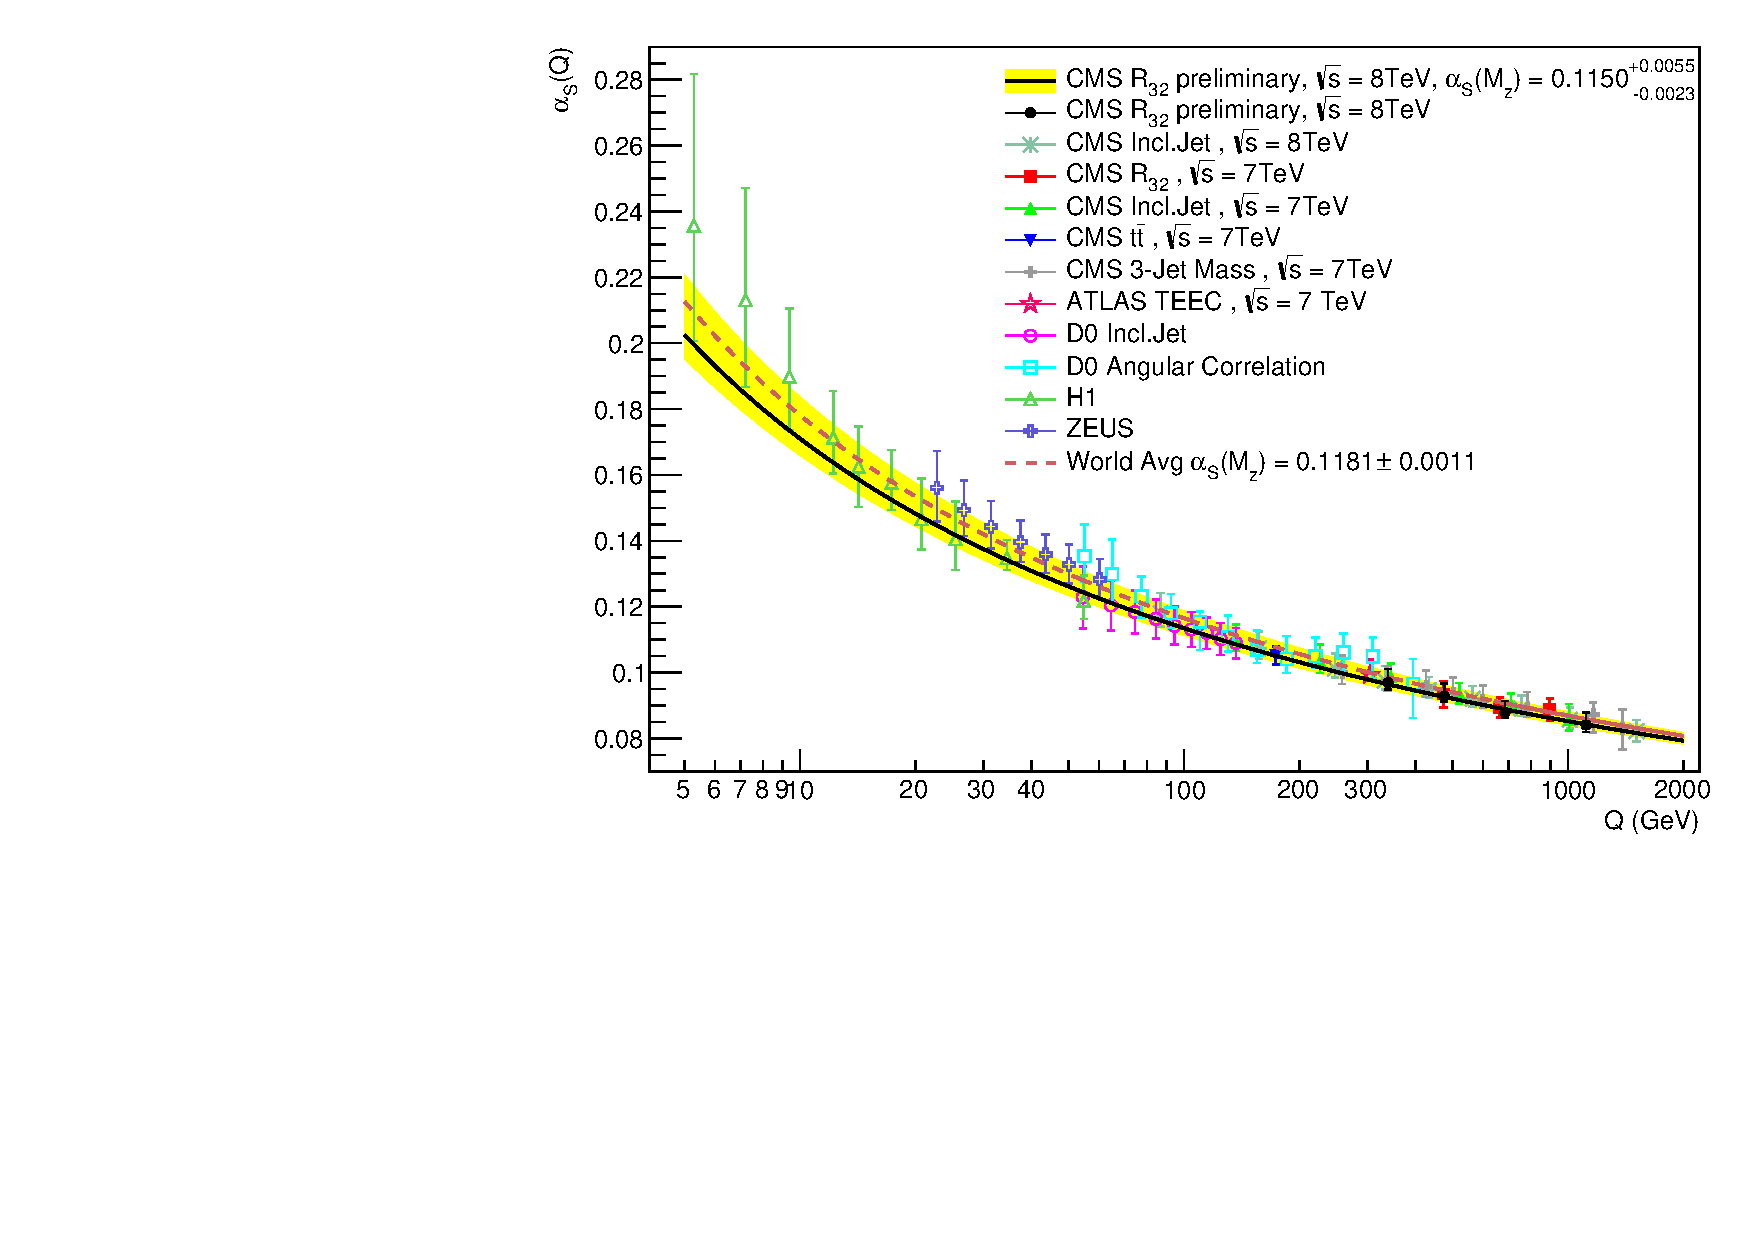
\includegraphics[width=1.05\textwidth]{Plots_HT_2_150/Running_alphas_8TeV_R32.pdf}\hftwo
  \caption{The running \alpsq as a function of the scale Q is shown as
    obtained by using the MSTW2008 NLO PDF set. The solid line and the
    uncertainty band are drawn by evolving the extracted \alpsmz
    values using the 2-loop 5-flavour renormalization group equations
    as implemented in \RunDec~\cite{Chetyrkin:2000yt,Schmidt:2012az}.
    The dashed line represents the evolution of the world
    average~\cite{Patrignani:2016xqp} and the black circles correspond
    to the \alpsq determinations presented in
    Table~\ref{tab:asq_values}. Results from other measurements of
    CMS~\cite{Chatrchyan:2013txa, Chatrchyan:2013haa,
      Khachatryan:2014waa, CMS:2014mna, Khachatryan:2016mlc},
    ATLAS~\cite{ATLAS:2015yaa}, D0~\cite{Abazov:2009nc,
      Abazov:2012lua}, H1~\cite{Andreev:2014wwa, Andreev:2016tgi}, and
    ZEUS~\cite{Abramowicz:2012jz} are superimposed.}
  \label{fig:running_alphas}
\end{figure}
